\graphicspath{{chapters/contents/sessio_01/images/}}

\section{Sessió 01 (14/09/26). Solucions.}
\subsection{Nivell I. Aigua bullint.}

\begin{figure}[H]
    \centering
    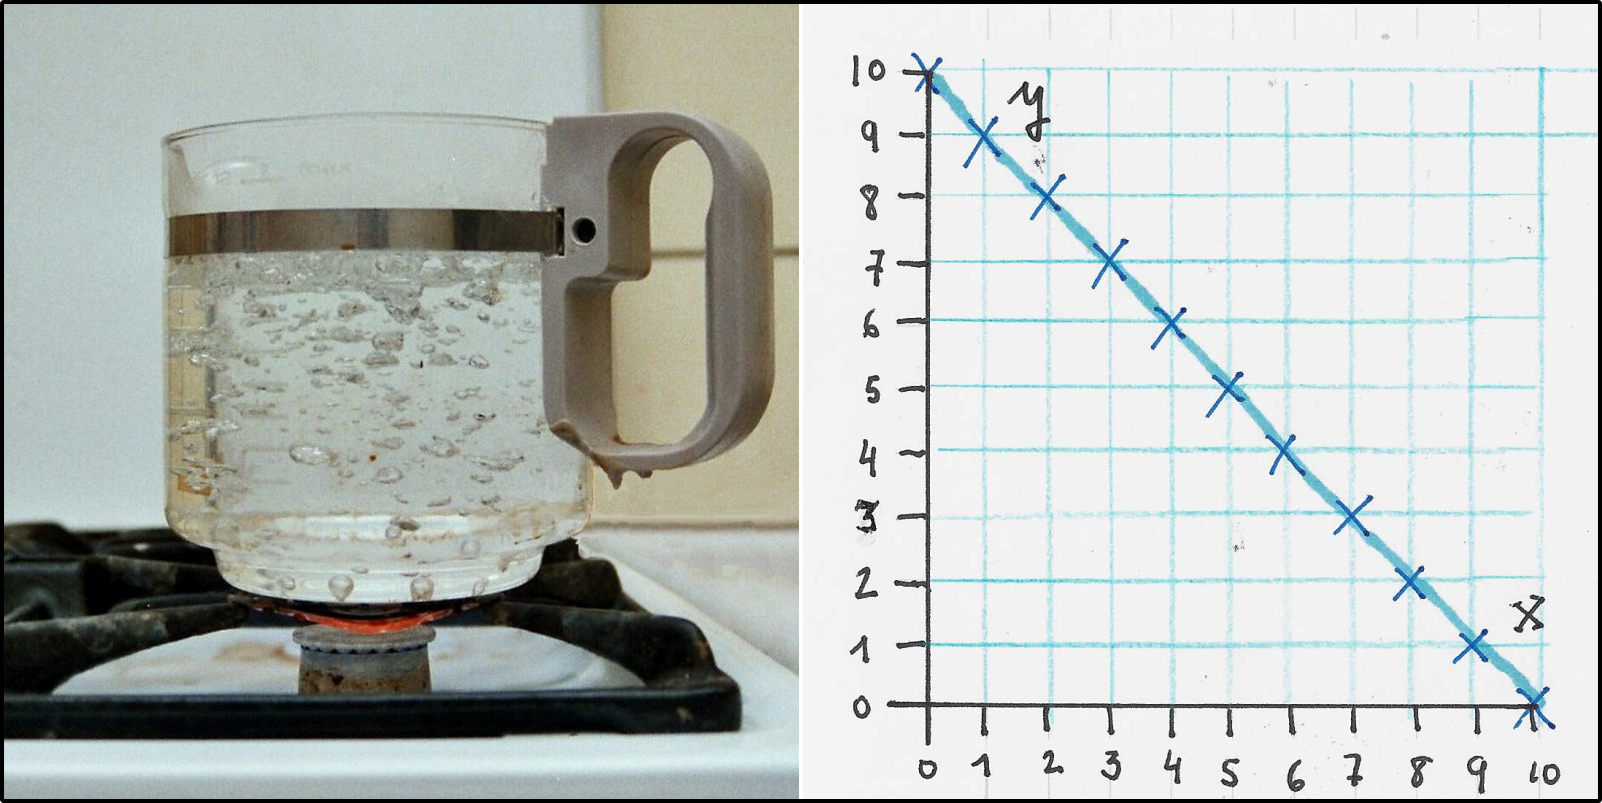
\includegraphics[width=1\linewidth]{actividad_1.png}
    \caption{\textit{Si mesuréssim la quantitat d’aigua que queda en un recipient mentre bull, podríem obtenir una gràfica com aquesta.} — Foto: Markus Schweiss — Wikimedia Commons, Wikimedia Commons, CC BY-SA 3.0.}
\end{figure}
L’equació que descriu exactament aquestes dades és
\[
y=10-x
\]
Podria representar els litres d’aigua que queden en un recipient a mesura que passa el temps. Si \(x\) són hores i \(y\) són litres, comencem amb 10 litres i en perdem aproximadament 1 cada hora.

Per aconseguir una cosa semblant en un experiment hauríem de mantenir l’aigua bullint i aportar una potència aproximadament constant, de l’ordre de 800--1000 W. Ja investigarem amb calma què és exactament això dels watts.

De moment, queda’t amb la idea important: cada vegada que \(x\) augmenta una unitat, \(y\) disminueix sempre la mateixa quantitat.

\newpage
\subsection{Nivell I. Muntanya russa.}

\begin{figure}[H]
    \centering
    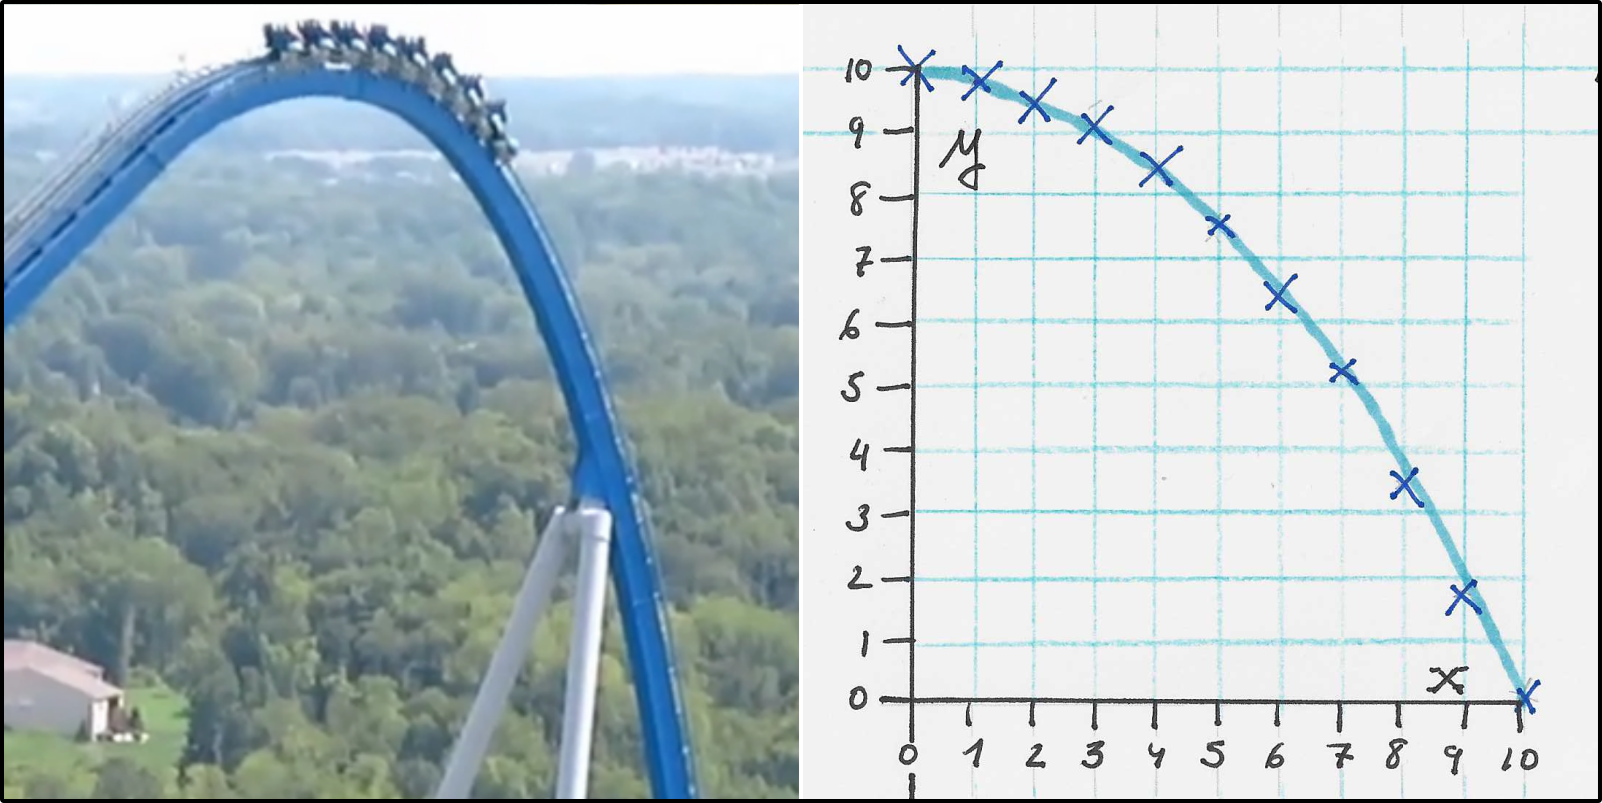
\includegraphics[width=1\linewidth]{actividad_2.png}
    \caption{\textit{La muntanya russa comença perdent altura molt a poc a poc, però a mesura que agafa velocitat baixa cada vegada més ràpidament.} — Foto: Airtime Thrills Raw Footage — Wikimedia Commons, CC BY-SA 4.0.}
\end{figure}

L’equació que encaixa exactament amb les dades és
\[
y=10-0.1x^2
\]
Podria representar l’altura respecte del terra d’un petit vagó que deixem baixar per una pendent. Pensa en una muntanya russa: quan comences la baixada encara vas lent i perds altura a poc a poc; cap al final ja portes força velocitat i l’altura disminueix molt més ràpidament, cosa que probablement la teva panxa ja s’haurà encarregat d’explicar-te.

Quan sapiguem resoldre problemes de moviment podrem comprovar que, fent algunes simplificacions, aquesta equació correspondria a una pendent d’uns 10 metres d’altura i uns 70 metres de longitud. Intenta dibuixar-la: com a muntanya russa no sembla especialment amenaçadora.

El que ens interessa ara és observar la forma de la gràfica. Al principi l’altura canvia poc, però després cau cada vegada més de pressa perquè el vagó va augmentant la velocitat.

\newpage
\subsection{Nivell I. La pilota voladora}

\begin{figure}[H]
    \centering
    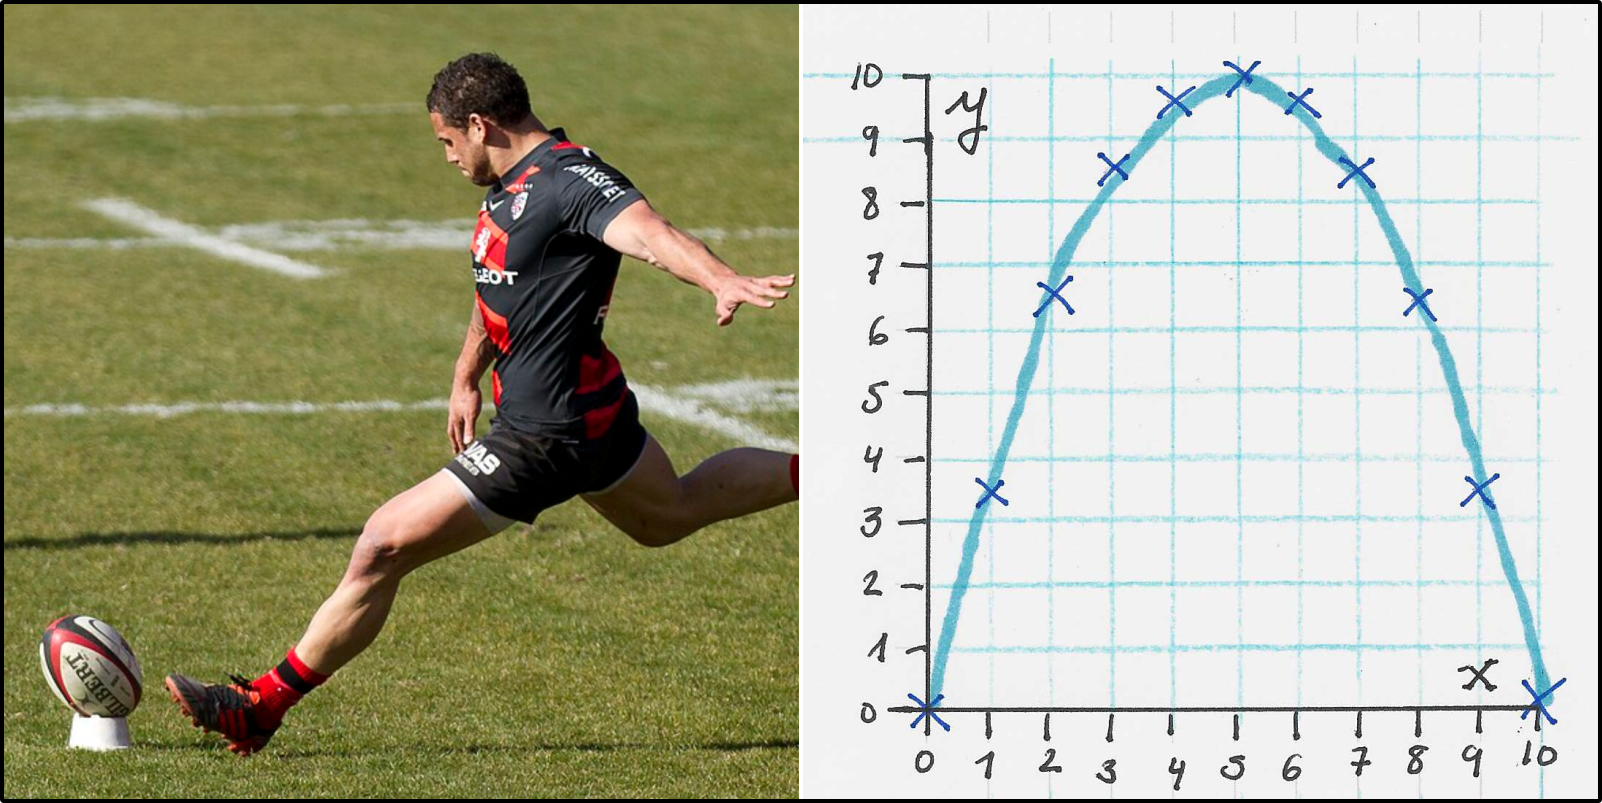
\includegraphics[width=1\linewidth]{actividad_3.png}
    \caption{\textit{Quan sapiguem una mica més de moviment podrem treure molta més informació de la mateixa corba. Per exemple, per obtenir aquesta trajectòria hauríem de xutar la pilota aproximadament a \(14.4\ \text{m/s}\) que són uns 52 km/h.} — Foto: Pierre-Selim — Wikimedia Commons, CC BY-SA 4.0.}
\end{figure}

L’equació d’aquesta gràfica és
\[
y=4x-0.4x^2
\]
Aquí apareix per primera vegada una \textbf{paràbola}. Una pista per reconèixer-la és mirar l’equació: hi apareixen alhora \(x\) i \(x^2\). Aquesta combinació és la que dona a la corba la seva forma característica.

Podria representar bastant bé la trajectòria d’una pilota de futbol: surt del terra, arriba a una altura màxima de 10 metres i torna a caure al terra 10 metres més enllà.

L’angle de llançament hauria de ser d’uns \(76^\circ\). Pots intentar mesurar-lo directament sobre la gràfica amb un transportador d’angles. No et sortirà exactament \(76^\circ\), però ja estem començant a treure física d’un simple dibuix.

\newpage
\subsection{Nivell I. Llei de la palanca}

\begin{figure}[H]
    \centering
    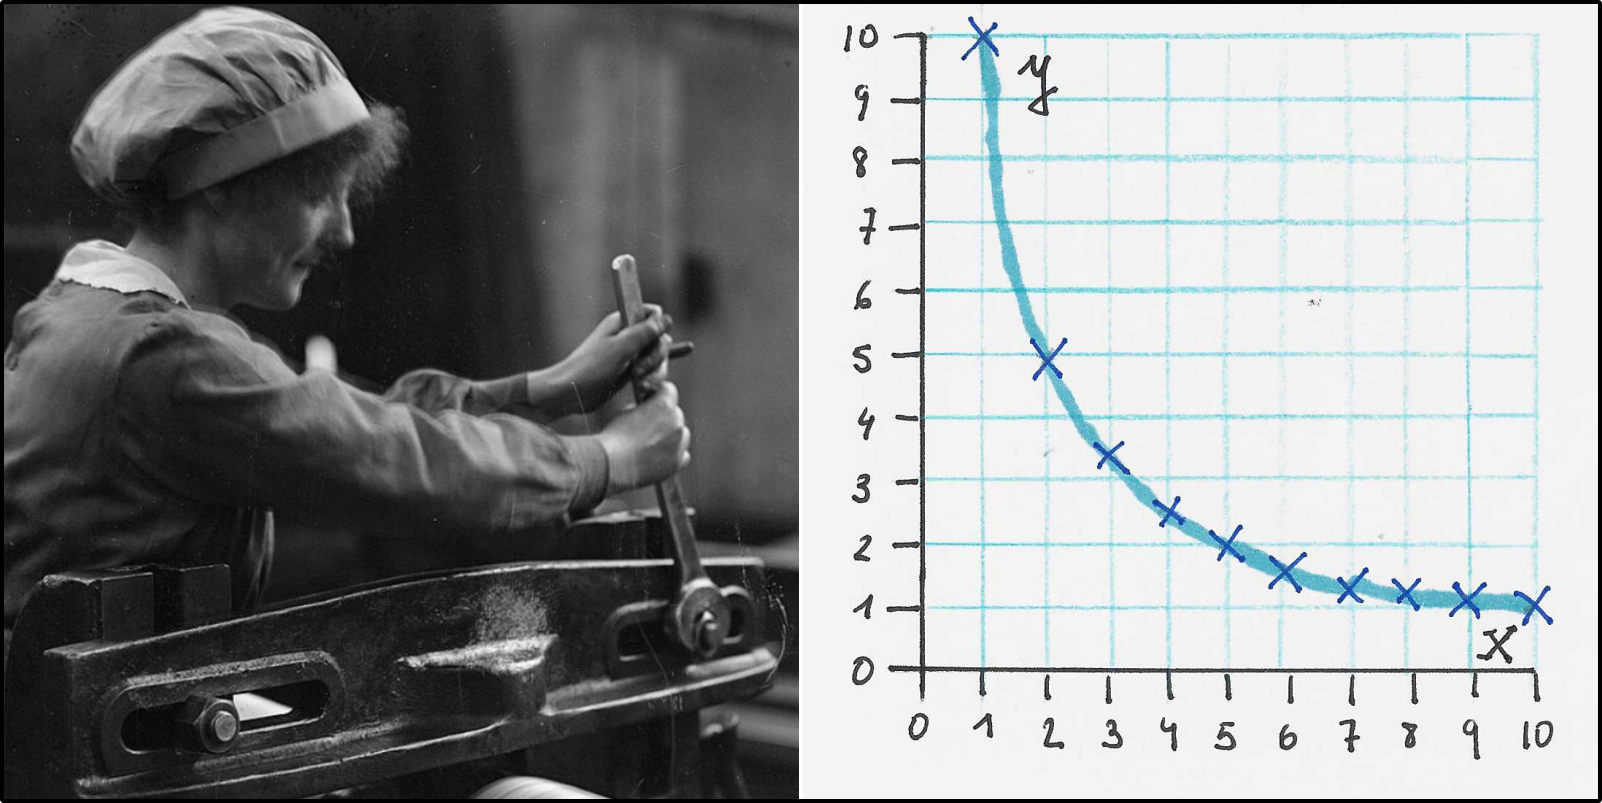
\includegraphics[width=1\linewidth]{actividad_4.png}
    \caption{\textit{Trobaríem aquest tipus de corbes si mesuréssim la força que cal fer amb una palanca, com ara una clau anglesa, a diferents distàncies de l’eix. Com més lluny apliquem la força, menys força necessitem fer.} — Foto: Wikimedia Commons, Public domain.}
\end{figure}

L’equació és
\[
y=\frac{10}{x}
\]
Aquest tipus de relació apareix quan, a mesura que una quantitat augmenta, l’altra disminueix de manera proporcional: si una es duplica, l’altra es redueix a la meitat.

Un exemple molt senzill és una palanca. Prova d’obrir una porta empenyent molt a prop de la frontissa i després des de la vora. Per aconseguir el mateix efecte, com més lluny ets de l’eix, menys força has de fer.

Podríem interpretar \(x\) com la distància a l’eix d’una clau i \(y\) com la força necessària per produir sempre el mateix efecte de gir. A més distància, menys força.

En física la força es mesura normalment en \textbf{newtons}. Ja veurem més endavant què significa exactament això i com es relaciona amb els «quilos» que fem servir de manera més informal quan parlem d’esforç o de pes.

Les relacions inverses apareixen en un munt de llocs: en el comportament dels gasos, en circuits elèctrics, en dissolucions... Definitivament, a la natura li agrada reutilitzar idees.

\newpage
\subsection{Nivell II. Una bola que es refreda.}

\begin{figure}[H]
    \centering
    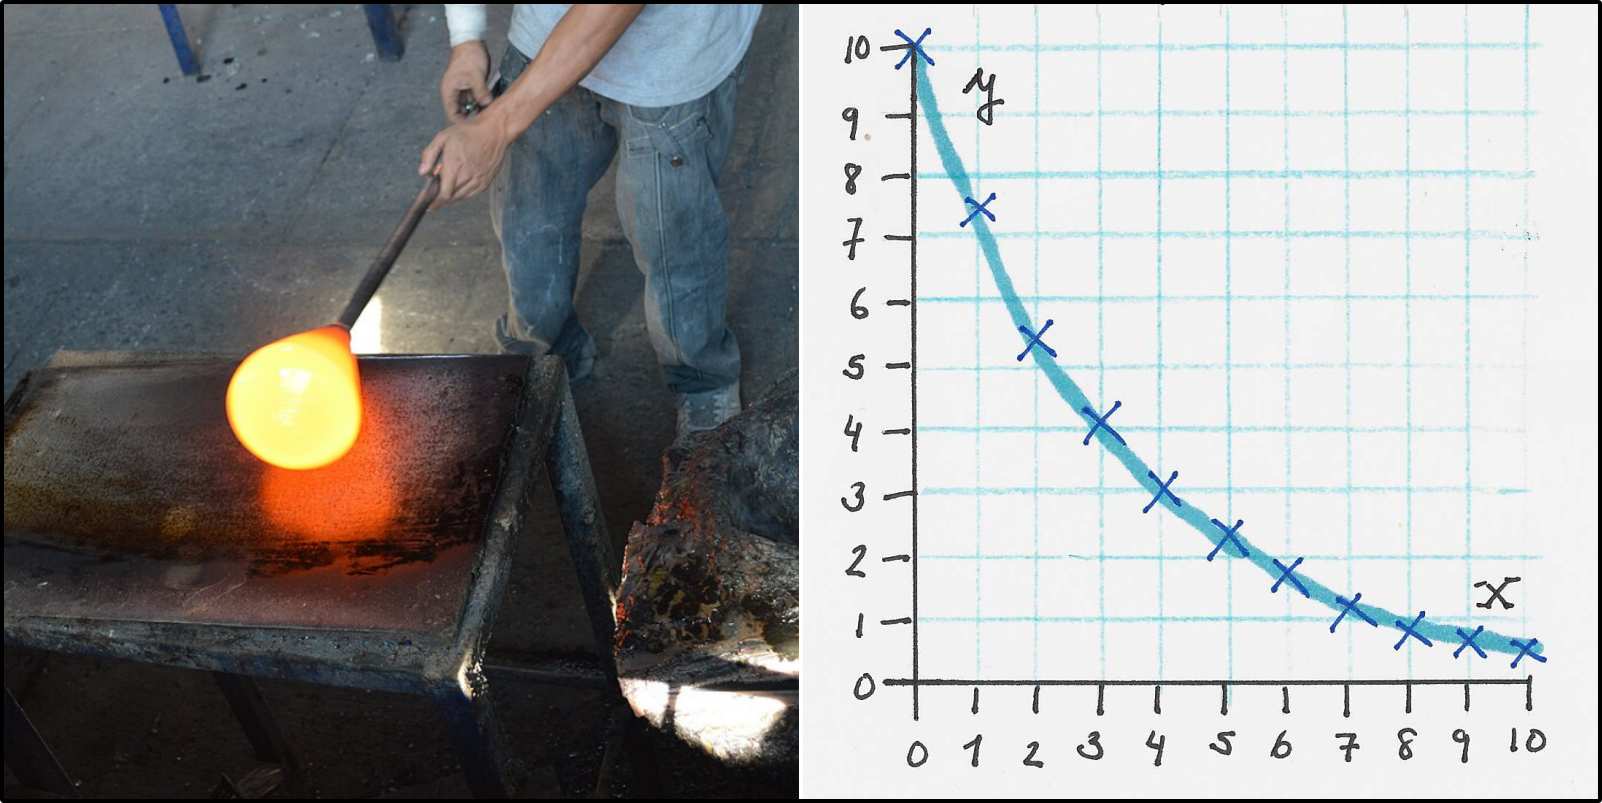
\includegraphics[width=1\linewidth]{actividad_5.png}
    \caption{\textit{A mesura que un objecte es refreda, la seva temperatura s’acosta a la de l’entorn. Al principi, com que la diferència de temperatura és gran, perd calor més ràpidament. A mesura que aquesta diferència es fa més petita, el refredament també es torna més lent.} — Foto: Alejandro Linares Garcia — Wikimedia Commons, CC BY-SA 3.0.}
\end{figure}

Les dades segueixen aproximadament aquesta equació:
\[
y=10e^{-0.3x}
\]
Aquí apareix una cosa nova: aquesta \(e\). Fins ara ens havíem apanyat bastant bé jugant amb \(x\), \(y\) i algunes potències, però per descriure aquest tipus de comportament això ja no és suficient. Necessitarem introduir alguns trucs matemàtics nous.

Aquesta \(e\) surt per tot arreu en física i té molt més significat del que sembla, però abans haurem d’afegir unes quantes eines a la nostra caixa d’eines matemàtiques. Així que, de moment, que ningú es ratlli amb ella.

Aquesta gràfica podria representar una petita esfera metàl·lica o ceràmica calenta que deixem refredar a l’aire. En aquest cas, \(y\) no representaria directament la temperatura de l’esfera, sinó la \textbf{diferència de temperatura respecte de l’ambient}.

Per exemple, si l’habitació està a 20~°C i \(y=10\), l’esfera estaria a 30~°C.

Podríem tenir que \(x\) sigui el temps en minuts i \(y\) els graus Celsius per sobre de la temperatura ambient. L’esfera comença 10~°C per sobre de la temperatura de l’ambient i s’hi va acostant a poc a poc. Observa que al principi es refreda ràpidament i després cada vegada més lentament.

A aquest comportament l’anomenarem \textbf{refredament exponencial}. Ja tindrem temps d’entendre bé la fórmula; ara ens interessa sobretot reconèixer la forma de la corba.

\newpage
\subsection{Nivell II. El moll posseït}

\begin{figure}[H]
    \centering
    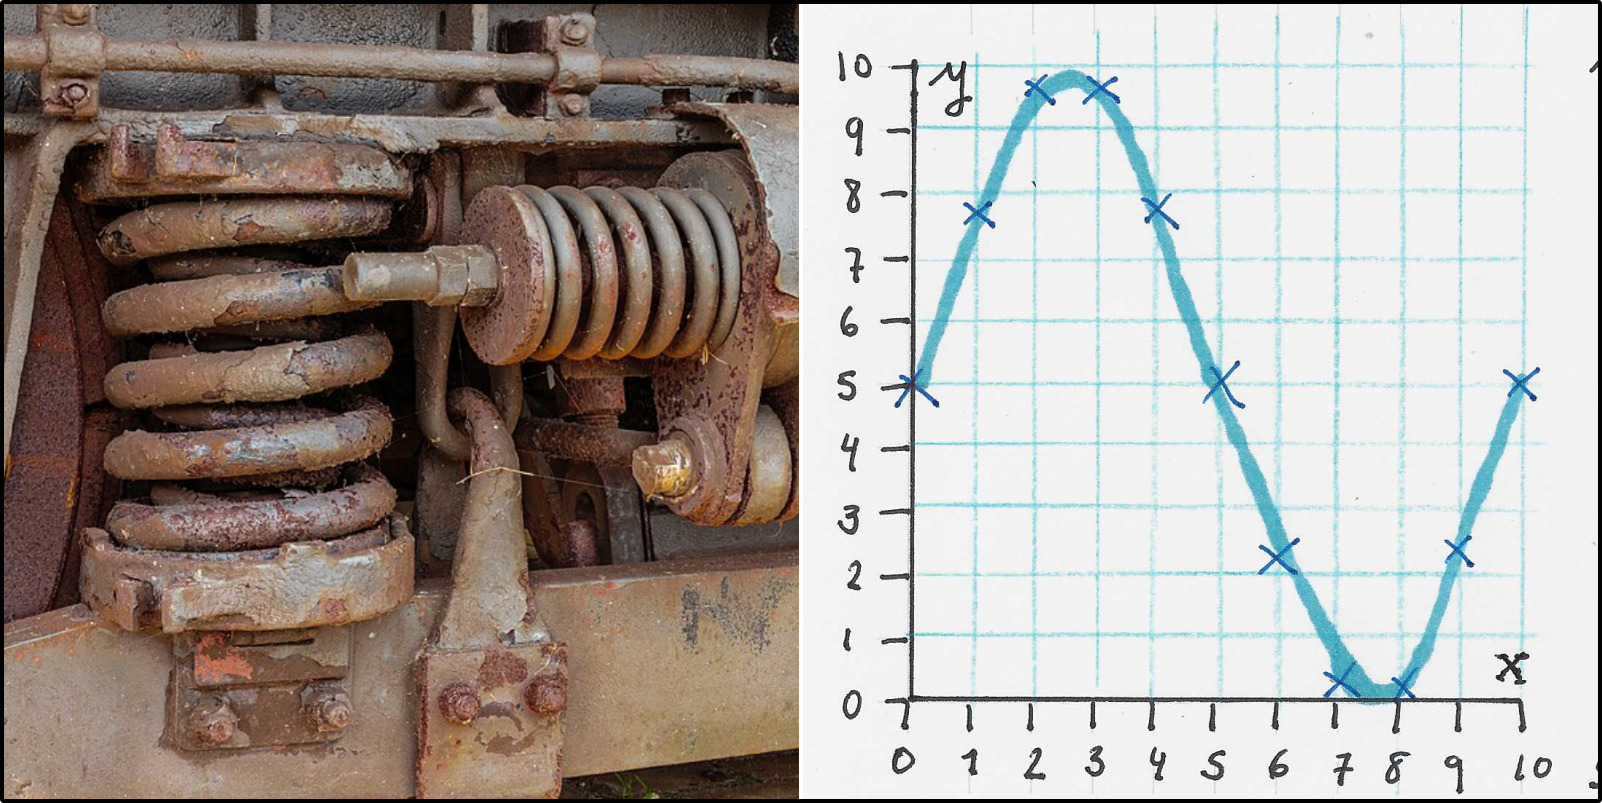
\includegraphics[width=1\linewidth]{actividad_6.png}
    \caption{\textit{Un moll pot oscil·lar més ràpid o més lent. La rapidesa de l’oscil·lació depèn sobretot de la seva rigidesa i de quanta massa hi carreguem. La mida, la forma, el material i el gruix del moll influeixen en aquesta rigidesa i, per tant, en la manera com oscil·la.} — Foto: Agnes Monkelbaan — Wikimedia Commons, CC BY-SA 4.0.}
\end{figure}


Aquestes dades encaixen gairebé perfectament amb el moviment d’una massa penjada d’un moll que oscil·la amunt i avall. L’equació és

\[
y=5+5\sin\left(\frac{\pi}{5}t\right)
\]

Aquí apareix una altra eina matemàtica nova: el \textbf{sinus}. No cal entendre encara d’on surt. De moment queda’t amb una idea: aquest tipus de corba apareix de manera natural quan alguna cosa oscil·la.

Podem interpretar \(x\) com el temps en segons i \(y\) com la posició de la massa en centímetres respecte d’una regla fixa.

La posició central és a 5 cm i la massa oscil·la 5 cm cap amunt i cap avall. Triga 10 dècimes de segon, és a dir, 1 segon, a completar una oscil·lació sencera.

Molls, pèndols, ones i moltes altres coses ens tornaran a portar a formes semblants.

\newpage
\subsection{Nivell Repte. La recta hi és, però s’ha de buscar}

\begin{figure}[H]
    \centering
    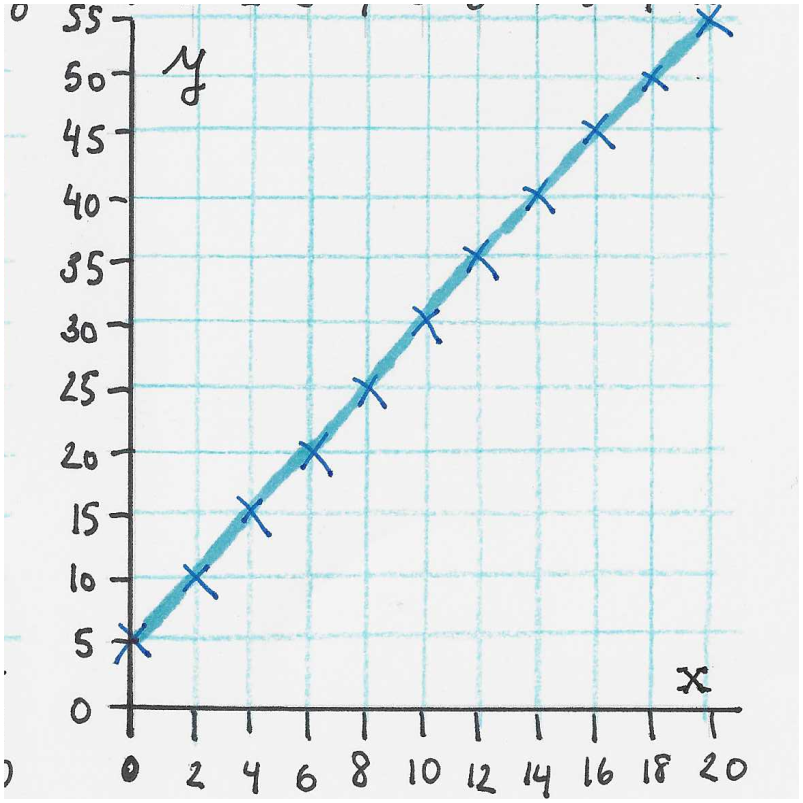
\includegraphics[width=1\linewidth]{actividad_7.png}
    \caption{\textit{A l’hora de representar les dades d’un experiment real, haurem d’ajustar l’escala perquè la gràfica ens càpiga al paper.}}
\end{figure}

L’equació continua sent una recta:
\[
y=5+2.5x
\]
La dificultat aquí no és tant l’equació com representar correctament les dades.

En els exercicis anteriors havíem tingut força sort: gairebé tot anava de 0 a 10 i podíem fer una marca per cada unitat. En un experiment real les coses rarament són tan amables i tan considerades.

Aquí l’eix \(x\) arriba fins a 20 i l’eix \(y\) fins a 55. Si féssim servir sempre un centímetre per cada unitat, necessitaríem una fulla bastant generosa.

Per això haurem d’aprendre a triar una \textbf{escala}: decidir quant representa cada marca de l’eix. A més, l’escala de l’eix \(x\) i la de l’eix \(y\) no tenen per què ser iguals.

No estem canviant les dades ni fent trampes. Simplement busquem una manera raonable de fer que la gràfica càpiga al paper i es pugui llegir.

\newpage
\subsection{Nivell Repte. Una mesura real.}

\begin{figure}[H]
    \centering
    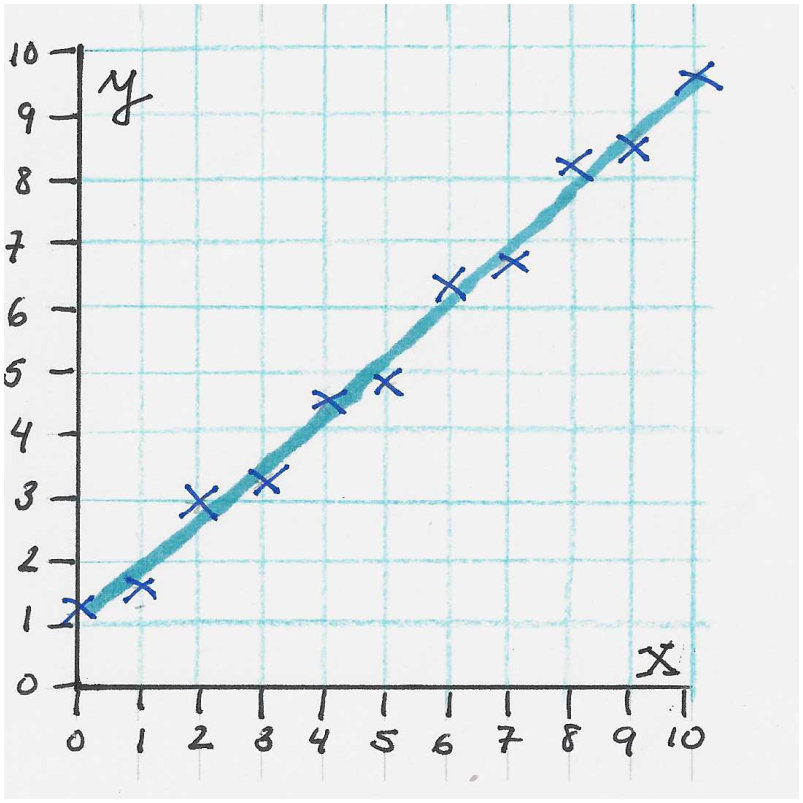
\includegraphics[width=1\linewidth]{actividad_8.png}
    \caption{\textit{No és que l’experiment hagi sortit malament, és que és molt difícil mesurar-ho tot amb total precisió i tenir-ho tot controlat.}}
\end{figure}

En aquest últim exercici passa una cosa molt més semblant al que trobarem en un laboratori de veritat: els punts no formen una recta perfecta.

Tot i això, semblen seguir aproximadament una relació del tipus
\[
y\approx0.85x+0.95
\]
Aquest símbol, \(\approx\), significa «aproximadament igual».

Que els punts no caiguin exactament sobre una recta no vol dir necessàriament que l’experiment hagi sortit malament. Les mesures reals tenen petites variacions, errors de mesura i altres factors que no sempre podem controlar.

Aleshores apareix una nova pregunta: si sembla que darrere de tots aquests punts hi ha una recta, quina recta triem?

No val simplement dibuixar la que ens sembli més bonica. Hi ha eines estadístiques que permeten trobar la recta que representa millor el conjunt de dades.

Ja hi arribarem. De moment, l’important és adonar-se d’una cosa bastant fonamental: en ciència les dades reals gairebé mai tenen l’educació de col·locar-se exactament on diu la fórmula.
